%###
\subsection{Einleitung}
%###
\label{sec:fachkonzept-usecase-einleitung}
\autorbeginn{Julia}

Um einen Überblick über die Funktionen zu bekommen, die das Planspiel abdecken sollen, wurde das folgende UseCase Diagramm auf \vref{img:fachkonzept-usecase} erstellt. In diesem Diagramm gibt es zwei Akteure, der Spielleiter und der Spieler. Die einzelnen Funktionen der beiden Akteure werden in den beiden folgenden Kapiteln näher erläutert.

\begin{figure}[htb]
  \centering
  \fbox{
    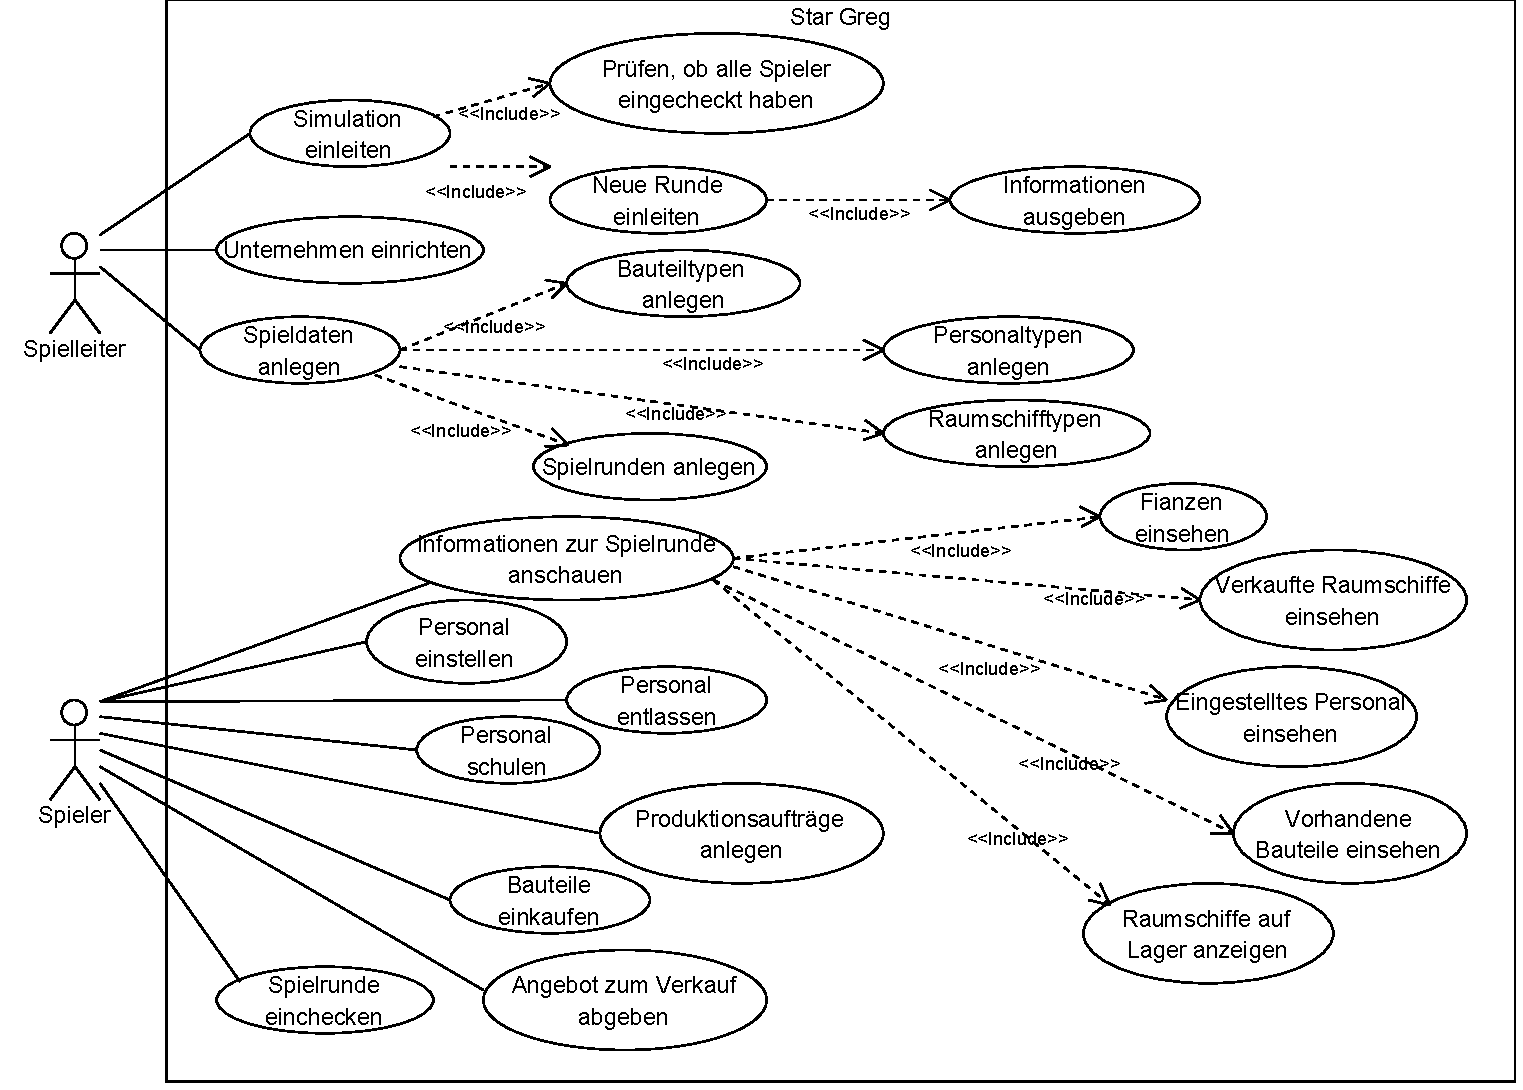
\includegraphics[width=0.9\textwidth]{30_Fachkonzept/10_UseCase/10_einleitung/diagramm}
  }
  \caption{UseCase Diagramm}
  \label{img:fachkonzept-usecase}
\end{figure}

\autorende{}